
\chapter{Estado del arte}
\label{cap:estado}

En este capítulo introduciremos el estado del arte en el mundo de la extrusión de filamentos. Más en concreto, veremos las varieades que hay en cuanto a la elección de una extrusora y el sistema de adquisició de datos que incorpora. Vamos a ver distintas empresas líderes en el mercado y las soluciones que ofrecen

\section{Rondol}

\begin{figure}[H]
    \centering
    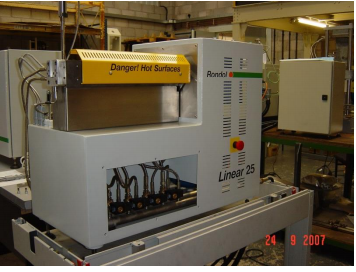
\includegraphics[width=0.6\textwidth]{images/rondol.png}
    \caption[Extrusora de laboratorio Linear 25]{Extrusora de laboratorio Linear 25. Fuente \cite{rondol}}
    \label{fig:rondol}.
\end{figure}


\section{Brabender}

\begin{figure}[H]
    \centering
    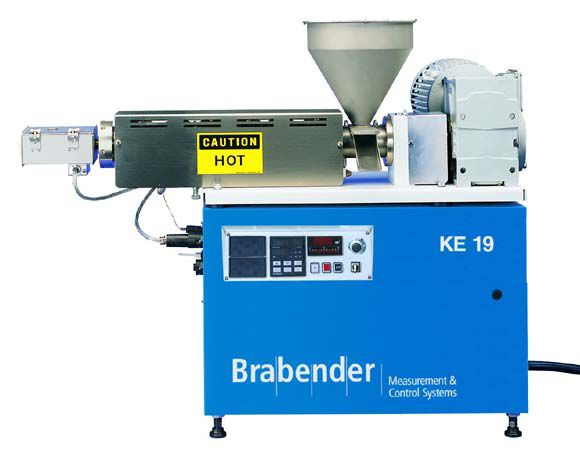
\includegraphics[width=0.6\textwidth]{images/brabender.jpg}
    \caption[Extrusora de laboratorio Stand-alone extruder KE 19]{Extrusora de laboratorio Stand-alone extruder KE 19. Fuente \cite{brabender}.}
    \label{fig:brabender}
\end{figure}

\section{Everplast}

\begin{figure}[H]
    \centering
    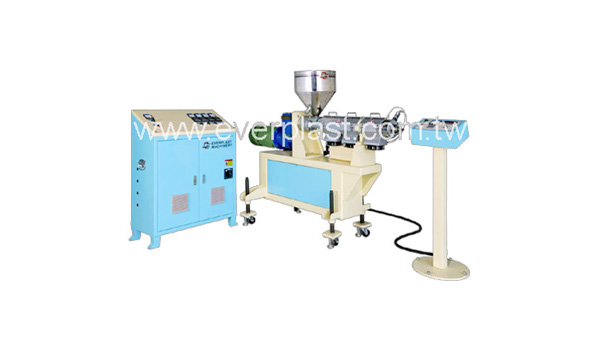
\includegraphics[width=0.7\textwidth]{images/everplast.jpg}
    \caption[Extrusora de laboratorio EMS-35]{Extrusora de laboratorioEMS-35. Fuente \cite{everplast}}
    \label{fig:everplast}
\end{figure}


\section{Extrusor Lyman}

En la actualidad, existen proyectos libres de extrusora de filamento que incorporan sistemas de control capaces de controlar los valores de la producción, como son el diámetro del filamento, temperaturas de trabajo y velocidades de extrusión y tracción \cite{lyman}. Ya que usan un microcontrolador para gestionar todo el proceso.\\


\begin{figure}[H]
    \centering
    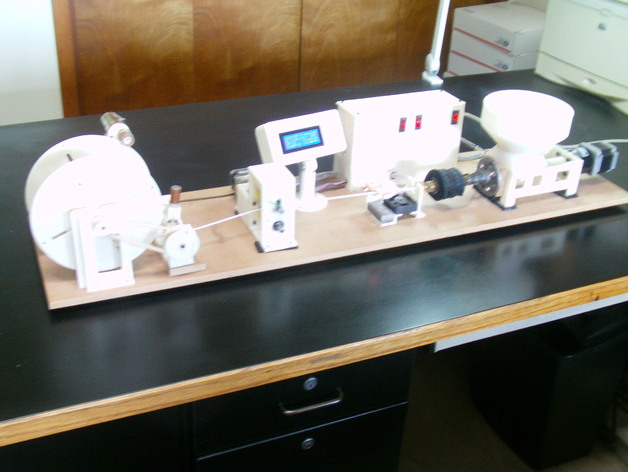
\includegraphics[width=0.7\textwidth]{images/lyman.jpg}
    \caption[Extrusora DIY Lyman extruder]{Extrusora DIY Lyman extruder. Fuente \cite{lyman}}
    \label{fig:lyman}
\end{figure}


Sin embargo, a pesar de que se podría incorporar, ninguno de ellos incorpora la capacidad de almacenar un registro con toda la información relevante de la producción. Ni tampoco un acceso remoto desde cualquier lugar del mundo. Por ello, el sistema que se propone realizar en este proyecto mejora las caracteríticas de estos sistemas.
